%!TEX TS-program = xelatex
%!TEX encoding = UTF-8 Unicode

\documentclass[11pt,tikz,border=1]{standalone}
\usetikzlibrary{positioning}

\begin{document}
  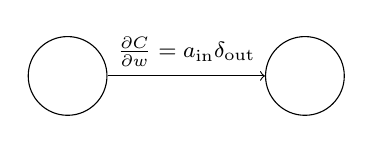
\begin{tikzpicture}[
    neuron/.style={circle,draw,inner sep=0pt,minimum size=10mm},
    font=\footnotesize
    ]

    \node(i) [neuron] {};
    \node(o) [neuron,right=2 of i] {};

    \draw[->] (i) -- node [above] {
      $\frac{\partial C}{\partial w} = a_{\rm in} \delta_{\rm out}$
    } (o);

  \end{tikzpicture}
\end{document}
